% chapter 3
\chapter{Analysis and Requirements}
Now that we have covered the relevant concepts needed, we shall proceed with
analysing the given problem, by creating an LP formulations that represent the problem to the highest possible accuracy.
The formulation section is followed by sections that analyses the approaches to solve the problem and its computational
complexity. Finally, we identify the requirements for furnish based on the analysis made in the previous sections. The
requirements are used to measure the success of our analysis.

\section{Problem Statement}
Furnish ltd\footnote{not a real company} is a leading furniture store with outlets that spread across the UK. In one busy day, the company is scheduled to
make deliveries to 226 customers across the country. The deliveries are made to the customers' location by delivery vehicles. All vehicles are
expected deliver all of the customers' goods in one visit.  There are 16 of these vehicles and they are based in
one central location (depot), where the company's goods are stored. The delivery vehicles only operate on
a time window from 09:00 to 17:00. On each delivery to a customer, it takes an average of 15 minutes for the workers to successfully unload the goods.
The company wants to find the routes that yield the minimum (optimal) distance and such that all customers are visited only once. They are interested
in finding the vehicle routes that yield the minimum distance for both with and without the time windows.
In addition, Furnish wants to find out if it can use less vans to make all deliveries while
keeping the total distance roughly the same as deliveries with 16 vehicles. The vehicles may serve up to 50 customers in a single tour.

We may make the following assumptions for convenience in modelling the LP formulations:
\begin{enumerate}
\item The service time for all deliveries is set to 15 minutes.
\item All vans are homogeneous and have very large capacity (up to 50 items).
\item Customers must receive all of their goods in a single visit, so we may set all customers' demand to 1.
\item The cost of function is set as the distance travelled.
\item Distance from one point to another may be calculated using the euclidian formula. We will use the haversine
formula\footnote{Refer to wikipedia for this} to convert it into real distance in km.
\item Traffic conditions are negligible and we assume that the roads from one point to another are straight.
\end{enumerate}

In addition to solving their vehicle routing problem, they have recently opened a new operations department to deal with the routing problem
 and would like a recommendation on which LP tool to use for their vehicle routing problem. The members of the team are
 mathematically competent but have very little experience with LP. Since this department is still in its
 experimental phase, its budget is minimum.

\section{Mathematical Formulation}
The problem stated in the previous section is known as the vehicle routing problem (VRP) \cite{Dantzig1959, Daneshzand2011},
a classic optimisation problem that has been documented and researched for decades. It is a problem where a fleet of vehicles,
which are based on a central location (also known as the depot), are required to visit geographically dispersed customers
 to fulfil their respective requirements. The main objective is to find the optimal routes for the fleet of vehicles that
 yield the minimum cost, which could be in terms of fuel, time or distance. There are many variants of VRP and they are based
 on the constraints imposed onto them. A few examples include VRP with multiple depot (MDVRP) \cite{Daneshzand2011} and a VRP where the
 customers can demand or return services (VRPB) \cite{Daneshzand2011}.
\begin{figure}[!ht]
  \centering
    \includegraphics[width=0.6\textwidth]{vrp-sample.png}
    \caption{A visualisation of VRP, taken from Networking and Emerging Optimization \cite{neo:vrp}}
\end{figure}

We can specifically define the problem given in the previous section with two known VRP models: capacitated
vehicle routing problem (CVRP) \cite{Daneshzand2011} and capacitated vehicle routing problem
with time windows model (CVRPTW) \cite{Daneshzand2011, Desrochers1988}. The CVRP model has the following input:
\begin{itemize}
\item A complete graph \(G = (V, E)\). which consists of the vertices \(V\) and the edges \(E\).
\item The variable \(n\), which represent the total number of customers and the depot.
\item The variable \(K\), which represent the total number of vehicles available. This will dictate the number of routes
generated in the model, with each vehicle having its own route.
\item A vertex set \(V\), numbered from 1 to \(n\) and vertex 1 is the depot.
\item A set of edges for \(V\).
\item The cost function \(c_{ij}\) that outputs the distance travelled from vertex i to j, where \(i,j \in V\).
\item The path function \(x_{ij}\) that outputs 1 if the path i to j is included in the current journey and 0 otherwise.
\item The capacity function \(r(S)\) that outputs the number capacity needed to serve a set of customers \(S\).
\end{itemize}

Given the input above, we can create a single depot capacitated vehicle routing problem below:

\vspace{0.5cm}

\begin{equation}
    \begin{array}{ll@{}ll}
        \text{Minimize} & \displaystyle\sum\limits_{i \in V}\sum\limits_{j \in V} c_{ij}&x_{ij} &\\
    \end{array}
\end{equation}
\begin{equation}
    \begin{array}{ll@{}ll}
        \text{Subject to}&\displaystyle\sum\limits_{i \in V}   &x_{ij} = 1,  &\forall j \in V \setminus \{1\}\\
    \end{array}
\end{equation}
\begin{equation}
    \begin{array}{ll@{}ll}
        & \displaystyle\sum\limits_{j \in V}   &x_{ij} = 1,  &\forall i \in V \setminus \{1\}\\
    \end{array}
\end{equation}
\begin{equation}
    \begin{array}{ll@{}ll}
        & \displaystyle\sum\limits_{i \in V}   &x_{1i} = K\\
    \end{array}
\end{equation}
\begin{equation}
    \begin{array}{ll@{}ll}
        & \displaystyle\sum\limits_{i \in V}   &x_{i1} = K\\
    \end{array}
\end{equation}
\begin{equation}
    \begin{array}{ll@{}ll@{}ll}
        & \displaystyle\sum\limits_{i \in S}\sum\limits_{i \in S}  &x_{ij} \leq |S| - r(S), &\forall S \subseteq V/ \{1\} , S \neq \o \\
    \end{array}
\end{equation}
\begin{equation}
    \begin{array}{ll@{}ll@{}ll}
        & x_{ij} = \{0,1\}\\
    \end{array}
\end{equation}

\vspace{1cm}

Equations (3.2) and (3.3) are constraints to ensure that all cities are visited only once, excluding the depot. Constraints (3.4) and (3.5)
impose the vehicles coming in must be equal to the vehicles coming out of the depot. Constraint (3.6) is the Subtour
Elimination Constraint (SEC) to ensure that each route taken by the vehicle is a hamiltonian cycle. Subtours are cycles that exist within set of vertices that causes
that partition the set into two or more components. Figures 3.2a and 3.2b illustrates the difference between a graph with subtours and a graph with a hamiltonian cycle.

There are two common formulations to eliminate subtours: the MTZ formulation by Miller et al \cite{Miller1960} and
the Subtour Formulation \cite{Lawler1985, Pataki2003}. Pataki \cite{Pataki2000} states that Subtour Elimination is the efficient formulation to reach optimal solution, whereas
the MTZ Formulation is highly inefficient despite its elegance. We formulate constraint (3.6) by combining capacity cut constraint (CCC), a constraint to ensure
that the vehicles meet the demands of all customers in a tour, with the Subtour Formulation to get the SEC for VRP \cite{Daneshzand2011}.
The SEC is essentail in producing the optimal routes in our VRP formulation.

\vspace{0.5cm}
\begin{figure}[!ht]
  \centering
    \begin{subfigure}{.5\textwidth}
      \centering
        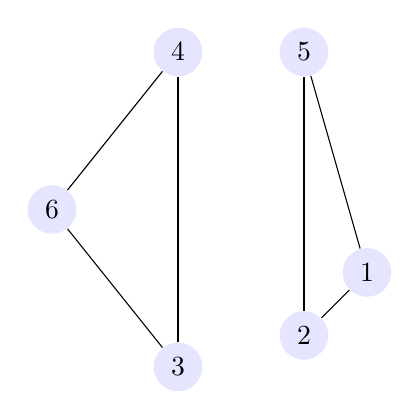
\begin{tikzpicture}
          [scale=.4,every node/.style={circle,fill=blue!10}]
          \node (n6) at (1,10) {6};
          \node (n4) at (5,15)  {4};
          \node (n5) at (9,15)  {5};
          \node (n1) at (11,8) {1};
          \node (n2) at (9,6)  {2};
          \node (n3) at (5,5)  {3};

          \foreach \from/\to in {n6/n4,n5/n1,n1/n2,n2/n5,n3/n4,n6/n3}
            \draw (\from) -- (\to);

        \end{tikzpicture}

      \caption{A graph with subtours}
      \label{fig:subtour}
    \end{subfigure}%
    \begin{subfigure}{.5\textwidth}
      \centering
      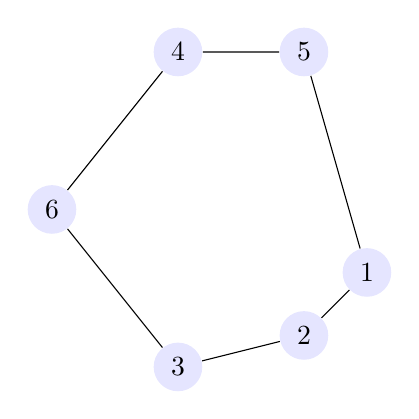
\begin{tikzpicture}
          [scale=.4,every node/.style={circle,fill=blue!10}]
          \node (n6) at (1,10) {6};
          \node (n4) at (5,15)  {4};
          \node (n5) at (9,15)  {5};
          \node (n1) at (11,8) {1};
          \node (n2) at (9,6)  {2};
          \node (n3) at (5,5)  {3};

          \foreach \from/\to in {n6/n4,n5/n1,n4/n5,n1/n2,n6/n3,n3/n2}
            \draw (\from) -- (\to);

        \end{tikzpicture}
      \caption{A graph with a hamiltonian cycle}
      \label{fig:hamiltoniancycle}
    \end{subfigure}
    \caption{A comparison of graph with identical vertices, one with subtours and the other with a hamiltonian cycle}
    \label{fig:subtourillus}
\end{figure}

In order to model CVRPTW, we need to introduce a new set of input related to time window constraints. We hold the assumptions made in the previous chapter.
\begin{itemize}
\item Variable \(D_{i}\) that represents the departure time to customer \(i\).
\item Time function \(t_{ij}\) that outputs the time taken to travel to customer \(i\) to \(j\).
\item Variable \(e_{i}\) that represents the earliest time for visiting customer \(i\).
\item Variable \(l_{i}\) that represents the latest time for visiting customer \(i\).
\item Variable \(y_{i}\) that represents the remaining capacity of the vehicle when visiting customer \(i\).
\item Variable \(q_{i}\) that represents the demand of customer \(i\).
\item Variable \(Q\) that represent the capacity of the vehicle \(i\).
\end{itemize}
Putting it together, we have the complete CVRPTW model below:

\vspace{0.5cm}

\begin{equation}
    \begin{array}{ll@{}ll}
        \text{Minimize} & \displaystyle\sum\limits_{i \in V}\sum\limits_{j \in V} c_{ij}&x_{ij} &\\
    \end{array}
\end{equation}
\begin{equation}
    \begin{array}{ll@{}ll}
        \text{Subject to}&\displaystyle\sum\limits_{i \in V}   &x_{ij} = 1,  &\forall j \in V \setminus \{1\}\\
    \end{array}
\end{equation}
\begin{equation}
    \begin{array}{ll@{}ll}
        & \displaystyle\sum\limits_{j \in V}   &x_{ij} = 1,  &\forall i \in V \setminus \{1\}\\
    \end{array}
\end{equation}
\begin{equation}
    \begin{array}{ll@{}ll}
        & \displaystyle\sum\limits_{i \in V}   &x_{1i} = K\\
    \end{array}
\end{equation}
\begin{equation}
    \begin{array}{ll@{}ll}
        & \displaystyle\sum\limits_{i \in V}   &x_{i1} = K\\
    \end{array}
\end{equation}
\begin{equation}
    \begin{array}{ll@{}ll@{}ll}
        & \displaystyle\sum\limits_{i \in S}\sum\limits_{i \in S}  &x_{ij} \leq |S| - r(S), &\forall S \subseteq V/ \{1\} , S \neq \o \\
    \end{array}
\end{equation}
\begin{equation}
    \begin{array}{ll@{}ll@{}ll}
        & x_{ij} = \{0,1\}\\
    \end{array}
\end{equation}
\begin{equation}
    \begin{array}{ll@{}ll@{}ll}
        & x_{ij} = 1 \implies D_{i} + t_{ij} \leq D_{j}, \forall i, j \in V / \{1\}
    \end{array}
\end{equation}
\begin{equation}
    \begin{array}{ll@{}ll@{}ll}
        & e_{i} \leq D_{i} \leq l_{i}, \forall i \in V / \{1\}
    \end{array}
\end{equation}
\begin{equation}
    \begin{array}{ll@{}ll@{}ll}
        & x_{ij} = 1 \implies y_{i} + q_{i} \leq y_{j}, \forall i, j \in V / \{1\}
    \end{array}
\end{equation}
\begin{equation}
    \begin{array}{ll@{}ll@{}ll}
        & 0 \leq y_{i} \leq Q, \forall i \in V / \{1\}
    \end{array}
\end{equation}

\vspace{1cm}

Constraint (3.15) ensures that given a chosen path from vertex i to j, the departure time of j does not exceed the
departure time at vertex i plus the time taken to travel from vertex i to j. Constraints (3.17) and (3.18) are the
demand and capacity constraints to ensure that the capacity does not exceed the demand at any point in the given route.

\section{Solution Methods}
Solution methods come in two categories: exact approaches and heuristics. Exact approaches attempt
to find the optimal solution and will not stop until it finds one of the best \cite{neo:exact}. Some examples
include branch-and-bound and the branch-and-cut algorithm \cite{here, ILPCoursera}. On the other hand, heuristics approach
 attempts to solve a problem more quickly at the expense of optimality and precision. Heuristics attempts to obtain the optimal solution by incrementally improve
 the current solution \cite{Laporte1999}. We use this technique in
solving problems that may take too long to compute the exact answer or when exact algorithms failed to find any solutio \cite{here}.
A few examples of these heuristics are sweep algorithm and tabu search.

The LP tools implement these algorithms and heuristics to find the optimal solution given a problem. Gurobi uses branch-and-bound method
to solve LP problems that contain integrality constraints \cite{gurobi:mip}. Whereas or-tools\footnote{this
is implied through the implementation of the solver. See \url{http://google.com}} and Optaplanner uses heuristics approach to solve VRP and other planning based
problems \cite{Optaplanner}.


\section{Requirements}
Based on our analysis and the goals of this project, we have identified a list of requirements needed to fulfill
their request / solve their problems. This will be used to benchmark the success of our analysis... Their respective
MoSCoW requirements are also included. They are tabulated in the list below:
\begin{enumerate}
\item Successfully model the LP formulations above - Must Have Priority
\item Compare and contrast LP tools - Should Have Priority
\item Give The optimal distance of the routes - must have
\item Give the optimal routes  - Must have
\item Give the optimal distance in KM - should have
\item Provide comments on the results - should have
\item Visualise the route on a map/graph - could haves
\end{enumerate}

\section{Review}
In this section we have...